% Options for packages loaded elsewhere
\PassOptionsToPackage{unicode}{hyperref}
\PassOptionsToPackage{hyphens}{url}
\documentclass[
]{article}
\usepackage[margin=0.75in]{geometry}
\usepackage{xcolor}
\usepackage{amsmath,amssymb}
\usepackage{graphicx}
\usepackage{pgfplots}
\pgfplotsset{compat=1.18}
\usepgfplotslibrary{fillbetween}
\usetikzlibrary{patterns}
\setcounter{secnumdepth}{-\maxdimen} % remove section numbering
\usepackage{iftex}
\ifPDFTeX
  \usepackage[T1]{fontenc}
  \usepackage[utf8]{inputenc}
  \usepackage{textcomp} % provide euro and other symbols
\else % if luatex or xetex
  \usepackage{unicode-math} % this also loads fontspec
  \defaultfontfeatures{Scale=MatchLowercase}
  \defaultfontfeatures[\rmfamily]{Ligatures=TeX,Scale=1}
\fi
\usepackage{lmodern}
\ifPDFTeX\else
  % xetex/luatex font selection
\fi
% Use upquote if available, for straight quotes in verbatim environments
\IfFileExists{upquote.sty}{\usepackage{upquote}}{}
\IfFileExists{microtype.sty}{% use microtype if available
  \usepackage[]{microtype}
  \UseMicrotypeSet[protrusion]{basicmath} % disable protrusion for tt fonts
}{}
\makeatletter
\@ifundefined{KOMAClassName}{% if non-KOMA class
  \IfFileExists{parskip.sty}{%
    \usepackage{parskip}
  }{% else
    \setlength{\parindent}{0pt}
    \setlength{\parskip}{6pt plus 2pt minus 1pt}}
}{% if KOMA class
  \KOMAoptions{parskip=half}}
\makeatother
\usepackage{longtable,booktabs,array}
\newcounter{none} % for unnumbered tables
\usepackage{calc} % for calculating minipage widths
% Correct order of tables after \paragraph or \subparagraph
\usepackage{etoolbox}
\makeatletter
\patchcmd\longtable{\par}{\if@noskipsec\mbox{}\fi\par}{}{}
\makeatother
% Allow footnotes in longtable head/foot
\IfFileExists{footnotehyper.sty}{\usepackage{footnotehyper}}{\usepackage{footnote}}
\makesavenoteenv{longtable}
\setlength{\emergencystretch}{3em} % prevent overfull lines
\providecommand{\tightlist}{%
  \setlength{\itemsep}{0pt}\setlength{\parskip}{0pt}}
\usepackage[backend=biber,style=authortitle,maxbibnames=99,doi=false,isbn=false,url=true]{biblatex}
\addbibresource{Analyzing_Late_20th_Century_Crime_Surge.bib}
\usepackage{bookmark}
\IfFileExists{xurl.sty}{\usepackage{xurl}}{} % add URL line breaks if available
\urlstyle{same}
\hypersetup{
  hidelinks,
  pdfcreator={LaTeX via pandoc}}

\author{Emmanuel Theodore}
\date{}

\begin{document}

\section{\texorpdfstring{\textbf{The Architecture of Violence: A
Multidimensional Framework Analysis of the Late Twentieth-Century Crime
Surge}}{The Architecture of Violence: A Multidimensional Framework Analysis of the Late Twentieth-Century Crime Surge}}\label{the-architecture-of-violence-a-multidimensional-framework-analysis-of-the-late-twentieth-century-crime-surge}

\subsection{\texorpdfstring{\textbf{Introduction}}{Introduction}}\label{introduction}

Between the early 1960s and the mid-1990s, the United States experienced
an unprecedented and sustained surge in violent crime. This period
fundamentally altered the American socio-political landscape, reshaping
urban geography, redefining law enforcement paradigms, and catalyzing
the exponential expansion of the carceral state. Understanding the
etiology of this surge requires moving beyond monolithic explanations
and embracing a multidimensional analytical approach. The crime wave was
not generated by a single variable, but rather by a complex confluence
of structural, environmental, demographic, and systemic factors. To
research the late twentieth-century violent crime surge through a
``frameworks lens'' is to acknowledge that violence is an output metric
generated by overlapping, interacting systems.\\
To deconstruct this phenomenon, this analysis synthesizes multiple
theoretical and empirical frameworks. Traditional sociological and
criminological models---such as social disorganization, general strain
theory, and routine activities theory---provide the foundational
behavioral context for understanding human action under pressure.
However, these models must be integrated with environmental diagnostics,
specifically the lead-crime hypothesis, as well as macro-economic
indicators documenting the collapse of industrial urban centers.
Furthermore, a rigorous analysis must account for the systemic
architecture of racialized spatial disadvantage, the proliferation of
illicit drug markets, demographic shifts, and the historical evolution
of the penal system from its Northern and Southern colonial roots. By
mapping the intersections of these variables, it becomes possible to
understand not only why violence escalated to historic peaks in the
early 1990s, but also how the subsequent political and legislative
responses---most notably the War on Drugs, Broken Windows policing, and
the Violent Crime Control and Law Enforcement Act of 1994---were
formulated in an environment of crisis, asymmetric choice, and systemic
extraction.

\subsection{\texorpdfstring{\textbf{The Empirical Topography of the
Crime
Surge}}{The Empirical Topography of the Crime Surge}}\label{the-empirical-topography-of-the-crime-surge}

Any rigorous analysis of the late twentieth-century crime wave must
begin with the empirical parameters of the surge. Crime data in the
United States is primarily tracked through two complementary systems:
the Federal Bureau of Investigation's Uniform Crime Reporting (UCR)
program, which tabulates offenses reported to law enforcement agencies,
and the Bureau of Justice Statistics' National Crime Victimization
Survey (NCVS), which captures both reported and unreported nonfatal
victimizations through randomized household surveys. Because the UCR
relies on police data, it is subject to the ``Hierarchy Rule,'' which
mandates that only the most serious offense in a multiple-offense
criminal incident be counted, with murder occupying the highest tier.\\
The UCR data reveals a stark, upward trajectory spanning three decades.
In 1960, the national homicide rate stood at 5.1 per 100,000 population,
with an estimated 9,110 homicides nationwide. Over the next two decades,
this rate doubled, peaking initially in 1980 at 10.2 homicides per
100,000 residents, accounting for 23,040 deaths. Following a brief
recession in the early 1980s, the homicide rate surged once more,
reaching a secondary peak of 9.8 per 100,000 in 1991, with nearly 24,703
homicides recorded that year. Correspondingly, the overall violent crime
rate---comprising murder, nonnegligent manslaughter, rape, robbery, and
aggravated assault---more than tripled between 1960 and 1991.

{\def\LTcaptype{none} % do not increment counter
\begin{longtable}[]{@{}
  >{\raggedright\arraybackslash}p{(\linewidth - 8\tabcolsep) * \real{0.2000}}
  >{\raggedright\arraybackslash}p{(\linewidth - 8\tabcolsep) * \real{0.2000}}
  >{\raggedright\arraybackslash}p{(\linewidth - 8\tabcolsep) * \real{0.2000}}
  >{\raggedright\arraybackslash}p{(\linewidth - 8\tabcolsep) * \real{0.2000}}
  >{\raggedright\arraybackslash}p{(\linewidth - 8\tabcolsep) * \real{0.2000}}@{}}
\toprule\noalign{}
\begin{minipage}[b]{\linewidth}\raggedright
Year
\end{minipage} & \begin{minipage}[b]{\linewidth}\raggedright
U.S. Population
\end{minipage} & \begin{minipage}[b]{\linewidth}\raggedright
Estimated Homicides
\end{minipage} & \begin{minipage}[b]{\linewidth}\raggedright
Homicide Rate (per 100,000)
\end{minipage} & \begin{minipage}[b]{\linewidth}\raggedright
Estimated Violent Crimes
\end{minipage} \\
\midrule\noalign{}
\endhead
\bottomrule\noalign{}
\endlastfoot
1960 & 179,323,175 & 9,110 & 5.1 & 288,460 \\
1965 & 193,526,000 & 9,960 & 5.1 & 486,750 \\
1970 & 203,265,212 & 16,000 & 7.9 & 738,820 \\
1975 & 213,124,000 & 20,510 & 9.6 & 1,039,710 \\
1980 & 225,349,264 & 23,040 & 10.2 & 1,344,520 \\
1985 & 238,740,000 & 18,976 & 7.9 & 1,328,800 \\
1991 & 252,177,000 & 24,703 & 9.8 & 1,911,770 \\
1995 & 262,755,000 & 21,606 & 8.2 & 1,798,790 \\
1999 & 272,690,813 & 15,522 & 5.7 & 1,426,044 \\
\end{longtable}
}

\emph{Data sourced from the FBI Uniform Crime Reports and BJS
Supplementary Homicide Reports, detailing the 1960-1999 trajectory.
Note: Violent crime estimates are derived from historical UCR volume
summaries.}

\begin{figure}[ht]
\centering
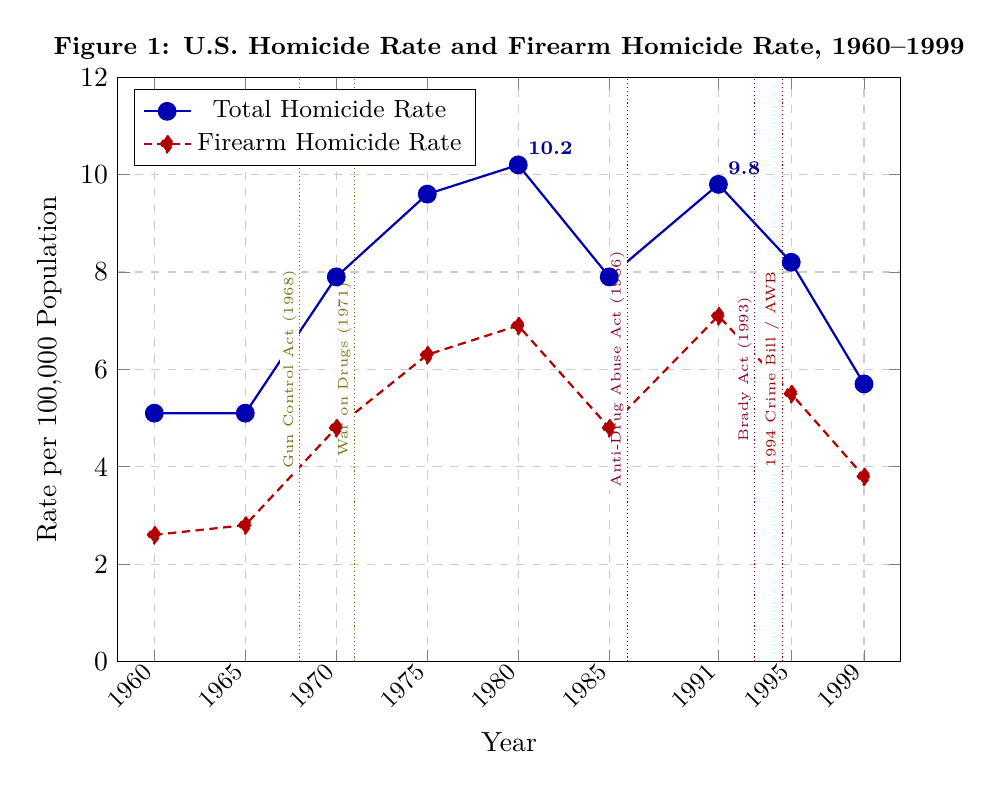
\begin{tikzpicture}
\begin{axis}[
    width=0.95\textwidth,
    height=9cm,
    xlabel={Year},
    ylabel={Rate per 100{,}000 Population},
    title={\textbf{Figure 1: U.S. Homicide Rate and Firearm Homicide Rate, 1960--1999}},
    xmin=1958, xmax=2001,
    ymin=0, ymax=12,
    xtick={1960,1965,1970,1975,1980,1985,1991,1995,1999},
    xticklabel style={rotate=45, anchor=east, font=\small, /pgf/number format/1000 sep={}},
    ytick={0,2,4,6,8,10,12},
    grid=major,
    grid style={dashed, gray!40},
    mark size=3pt,
    every axis title/.style={font=\bfseries\small, at={(0.5,1.05)}},
    legend style={at={(0.02,0.98)}, anchor=north west, font=\small},
]
\addplot[thick, blue!70!black, mark=*] coordinates {
    (1960, 5.1) (1965, 5.1) (1970, 7.9) (1975, 9.6)
    (1980, 10.2) (1985, 7.9) (1991, 9.8) (1995, 8.2) (1999, 5.7)
};
\addlegendentry{Total Homicide Rate}
\addplot[thick, red!70!black, mark=diamond*, densely dashed] coordinates {
    (1960, 2.6) (1965, 2.8) (1970, 4.8) (1975, 6.3)
    (1980, 6.9) (1985, 4.8) (1991, 7.1) (1995, 5.5) (1999, 3.8)
};
\addlegendentry{Firearm Homicide Rate}
% Peak annotations
\node[above right, font=\scriptsize, blue!60!black] at (axis cs:1980,10.2) {\textbf{10.2}};
\node[above right, font=\scriptsize, blue!60!black] at (axis cs:1991,9.8) {\textbf{9.8}};
% Policy event vertical lines with labels at mid-graph
\draw[densely dotted, olive!80!black] (axis cs:1968,0) -- (axis cs:1968,12);
\node[rotate=90, anchor=south, font=\tiny, olive!80!black, fill=white, inner sep=1pt] at (axis cs:1968,6) {Gun Control Act (1968)};
\draw[densely dotted, olive!80!black] (axis cs:1971,0) -- (axis cs:1971,12);
\node[rotate=90, anchor=south, font=\tiny, olive!80!black, fill=white, inner sep=1pt] at (axis cs:1971,6) {War on Drugs (1971)};
\draw[densely dotted, purple!70!black] (axis cs:1986,0) -- (axis cs:1986,12);
\node[rotate=90, anchor=south, font=\tiny, purple!70!black, fill=white, inner sep=1pt] at (axis cs:1986,6) {Anti-Drug Abuse Act (1986)};
\draw[densely dotted, purple!70!black] (axis cs:1993,0) -- (axis cs:1993,12);
\node[rotate=90, anchor=south, font=\tiny, purple!70!black, fill=white, inner sep=1pt] at (axis cs:1993,6) {Brady Act (1993)};
\draw[densely dotted, red!60!black] (axis cs:1994.5,0) -- (axis cs:1994.5,12);
\node[rotate=90, anchor=south, font=\tiny, red!60!black, fill=white, inner sep=1pt] at (axis cs:1994.5,6) {1994 Crime Bill / AWB};
\end{axis}
\end{tikzpicture}
\caption*{\emph{Sources: FBI Uniform Crime Reports; BJS Supplementary Homicide Reports; CDC WONDER Compressed Mortality File (firearm homicide). Policy events: Gun Control Act of 1968; Nixon's War on Drugs declaration (1971); Anti-Drug Abuse Act of 1986 (mandatory minimums, 100:1 crack/powder disparity); Brady Handgun Violence Prevention Act (1993); Violent Crime Control and Law Enforcement Act of 1994 (including Federal Assault Weapons Ban). Note: Firearm homicides consistently accounted for 60--70\% of all homicides throughout the surge, peaking at approximately 70\% in 1991.}}
\end{figure}

The NCVS data covering 1973 to 1995 confirms these volatile fluctuations
from the perspective of the victim. The survey identifies distinct
short-term trends within the broader surge: a period of stability from
1973 to 1977, rapid escalation to a peak in 1981, a temporary decrease
between 1981 and 1986, and a final, severe escalation from 1986 to 1993.
This late-1980s escalation was driven heavily by aggravated assaults and
robberies.\\
A critical transition during this era was the changing topological
nature of violent encounters. Historically, homicide and severe assault
were predominantly interpersonal crimes committed among acquaintances or
domestic partners. However, during the 1970s and 1980s, homicide rates
by strangers increased much faster than domestic homicides, particularly
in dense urban centers. Robberies, which frequently escalated into
stranger-on-stranger murder or severe injury, increased by a factor of
four between 1960 and 1980. This shift toward impersonal, unpredictable
violence in public spaces generated an unprecedented level of national
fear, fundamentally altering how Americans navigated urban environments.
Furthermore, a paradox emerged in the data: between 1973 and 1995, total
violent victimizations reported to the police by victims actually
decreased by 5\%, yet crimes recorded by the police rose by 116\%. This
narrowing gap is largely attributed to technological improvements in
police record-keeping systems, the proliferation of 911 dispatch
networks, and better reporting architectures between local agencies and
the FBI, meaning that the perception of the crime wave was amplified by
suddenly superior data capture.

\begin{figure}[ht]
\centering
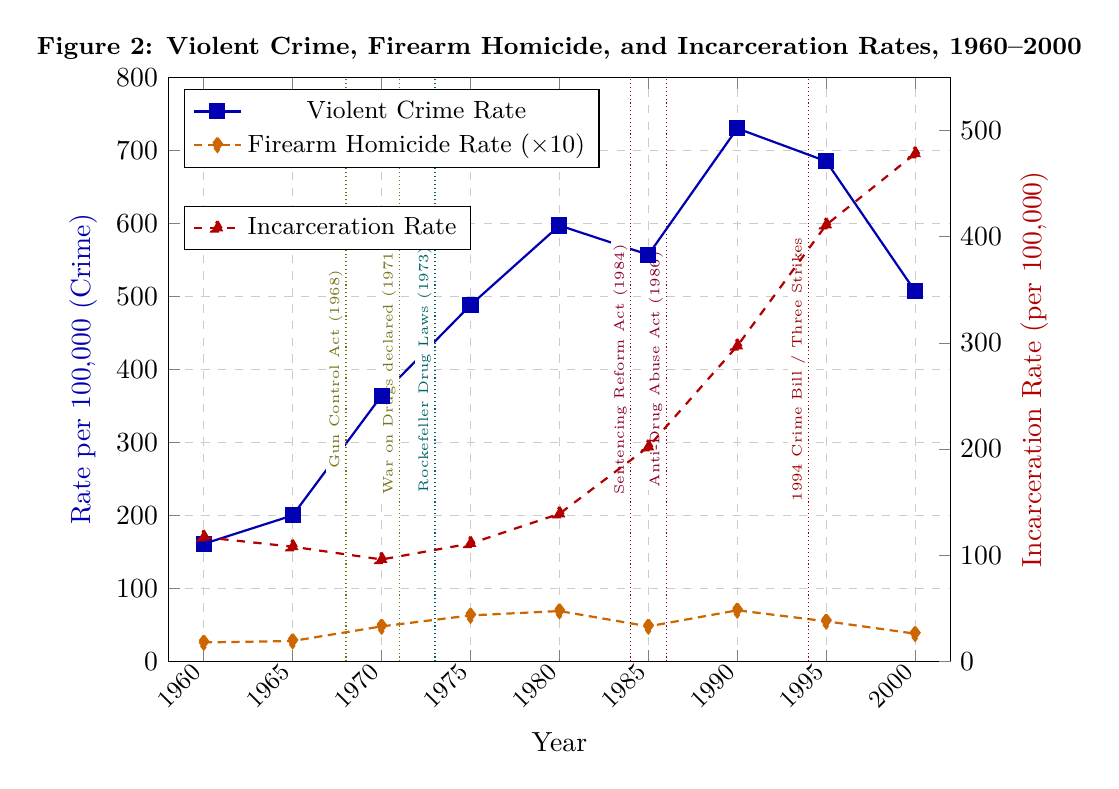
\begin{tikzpicture}
\begin{axis}[
    width=0.95\textwidth,
    height=9cm,
    title={\textbf{Figure 2: Violent Crime, Firearm Homicide, and Incarceration Rates, 1960--2000}},
    xlabel={Year},
    ylabel={Rate per 100{,}000 (Crime)},
    axis y line*=left,
    xmin=1958, xmax=2002,
    ymin=0, ymax=800,
    xtick={1960,1965,1970,1975,1980,1985,1990,1995,2000},
    xticklabel style={rotate=45, anchor=east, font=\small, /pgf/number format/1000 sep={}},
    grid=major,
    grid style={dashed, gray!40},
    ylabel style={blue!70!black},
    mark size=2.5pt,
    every axis title/.style={font=\bfseries\small, at={(0.5,1.05)}},
    legend style={at={(0.02,0.98)}, anchor=north west, font=\small},
]
\addplot[thick, blue!70!black, mark=square*] coordinates {
    (1960, 161) (1965, 200) (1970, 364) (1975, 488)
    (1980, 597) (1985, 557) (1990, 730) (1995, 685) (2000, 507)
};
\addlegendentry{Violent Crime Rate}
% Firearm homicide rate scaled x10 so it's visible on the same axis
\addplot[thick, orange!80!black, mark=diamond*, densely dashed] coordinates {
    (1960, 26) (1965, 28) (1970, 48) (1975, 63)
    (1980, 69) (1985, 48) (1990, 70) (1995, 55) (2000, 38)
};
\addlegendentry{Firearm Homicide Rate ($\times$10)}
% Policy event vertical lines with labels at mid-graph
\draw[densely dotted, olive!80!black] (axis cs:1968,0) -- (axis cs:1968,800);
\node[rotate=90, anchor=south, font=\tiny, olive!80!black, fill=white, inner sep=1pt] at (axis cs:1968,400) {Gun Control Act (1968)};
\draw[densely dotted, olive!80!black] (axis cs:1971,0) -- (axis cs:1971,800);
\node[rotate=90, anchor=south, font=\tiny, olive!80!black, fill=white, inner sep=1pt] at (axis cs:1971,400) {War on Drugs declared (1971)};
\draw[densely dotted, teal!80!black] (axis cs:1973,0) -- (axis cs:1973,800);
\node[rotate=90, anchor=south, font=\tiny, teal!80!black, fill=white, inner sep=1pt] at (axis cs:1973,400) {Rockefeller Drug Laws (1973)};
\draw[densely dotted, purple!70!black] (axis cs:1984,0) -- (axis cs:1984,800);
\node[rotate=90, anchor=south, font=\tiny, purple!70!black, fill=white, inner sep=1pt] at (axis cs:1984,400) {Sentencing Reform Act (1984)};
\draw[densely dotted, purple!70!black] (axis cs:1986,0) -- (axis cs:1986,800);
\node[rotate=90, anchor=south, font=\tiny, purple!70!black, fill=white, inner sep=1pt] at (axis cs:1986,400) {Anti-Drug Abuse Act (1986)};
\draw[densely dotted, red!60!black] (axis cs:1994,0) -- (axis cs:1994,800);
\node[rotate=90, anchor=south, font=\tiny, red!60!black, fill=white, inner sep=1pt] at (axis cs:1994,400) {1994 Crime Bill / Three Strikes};
\end{axis}
\begin{axis}[
    width=0.95\textwidth,
    height=9cm,
    axis y line*=right,
    axis x line=none,
    ylabel={Incarceration Rate (per 100{,}000)},
    xmin=1958, xmax=2002,
    ymin=0, ymax=550,
    ytick={0,100,200,300,400,500},
    ylabel style={red!70!black},
    mark size=2.5pt,
    legend style={at={(0.02,0.78)}, anchor=north west, font=\small},
]
\addplot[thick, red!70!black, mark=triangle*, dashed] coordinates {
    (1960, 117) (1965, 108) (1970, 96) (1975, 111)
    (1980, 139) (1985, 202) (1990, 297) (1995, 411) (2000, 478)
};
\addlegendentry{Incarceration Rate}
\end{axis}
\end{tikzpicture}
\caption*{\emph{Sources: FBI UCR violent crime data; CDC WONDER Compressed Mortality File (firearm homicide); Bureau of Justice Statistics, Prisoners Series; The Sentencing Project, ``Trends in U.S.\ Corrections.'' Policy events: Gun Control Act (1968); Nixon's War on Drugs (1971); Rockefeller Drug Laws (1973); Sentencing Reform Act (1984); Anti-Drug Abuse Act (1986); Violent Crime Control Act (1994). Note: Firearm homicide rate is scaled $\times$10 for visual comparability. The incarceration rate begins its steep ascent after the Sentencing Reform Act and Anti-Drug Abuse Act---precisely as violent crime plateaus and then declines.}}
\end{figure}

\clearpage

\subsection{\texorpdfstring{\textbf{Foundational Criminological
Frameworks}}{Foundational Criminological Frameworks}}\label{foundational-criminological-frameworks}

To explain the steep trajectory of these statistics, criminologists in
the late twentieth century leaned heavily on three major structural
theories: social disorganization, strain theory, and routine activities
theory. These frameworks departed from early positivist criminology,
which sought biological or phrenological causes for deviance, and
instead focused on the intersection of human rationality, social
structures, and environmental pressures.

\subsubsection{\texorpdfstring{\textbf{Social Disorganization
Theory}}{Social Disorganization Theory}}\label{social-disorganization-theory}

Originating from the Chicago School of Sociology in the early twentieth
century through the cartographic work of Clifford Shaw and Henry McKay,
social disorganization theory posits that crime is not merely the result
of individual pathology, but rather the product of neighborhood
ecological conditions. The theory suggests that stable neighborhoods
possess ``collective efficacy''---the mutual trust, social cohesion, and
willingness of residents to intervene for the common good and maintain
informal social control.\\
As urban centers underwent severe demographic and economic transitions
in the 1970s and 1980s, these localized social ties began to fray. High
residential turnover, extreme poverty, and the physical deterioration of
neighborhoods depleted collective efficacy. In areas lacking integrated
social networks and robust civic institutions, ``conflict'' subcultures
centered around violence rapidly emerged to fill the vacuum. The spatial
dimension of this theory proved highly predictive during the late 20th
century; crime did not rise uniformly across the United States, but
rather clustered violently in specific urban ecological zones where
traditional family structures, local economies, and institutional trust
had collapsed.

\subsubsection{\texorpdfstring{\textbf{Strain Theory and Relative
Deprivation}}{Strain Theory and Relative Deprivation}}\label{strain-theory-and-relative-deprivation}

Developed initially by Robert K. Merton and subsequently expanded by
Robert Agnew into General Strain Theory in 1992, this framework argues
that crime occurs when individuals experience a profound disconnect
between socially promoted cultural goals and the legitimate, structural
means to achieve them.\\
During the late twentieth century, structural inequality widened
dramatically in the United States. In a capitalist system that heavily
promotes material accumulation and associates status with wealth,
relative deprivation became a powerful criminogenic force. When
individuals in impoverished urban enclaves internalized the cultural
mandate for success but found the legitimate avenues (education, stable
employment) blocked by systemic barriers, they experienced intense
psychological strain. Agnew expanded this to include non-economic
strains, emphasizing that negative life events, chronic stress, removal
of positive stimuli, and the persistent trauma of racial discrimination
create psychological pressures that frequently manifest as delinquency,
anger, and violence when legitimate coping mechanisms are unavailable.
Therefore, the crime surge can be viewed as an adaptive, albeit
destructive, behavioral response to the intensification of structural
strain.

\subsubsection{\texorpdfstring{\textbf{Routine Activities Theory and
Rational
Choice}}{Routine Activities Theory and Rational Choice}}\label{routine-activities-theory-and-rational-choice}

Formulated by Lawrence Cohen and Marcus Felson in 1979, routine
activities theory provided a distinct, pragmatic lens that diverged from
sociological deep-structure arguments. This theory asserts that crime
rates correspond directly to changes in the daily routines of modern
life. It posits that a criminal event requires the precise spatial and
temporal convergence of three elements: a motivated offender, a suitable
target, and the absence of a capable guardian.\\
During the 1970s and 1980s, fundamental shifts in American lifestyle
radically altered these variables. The mass entry of women into the
workforce and increased residential mobility resulted in millions of
homes being left unattended during the day, drastically reducing capable
guardianship. Simultaneously, the proliferation of lightweight, easily
fenced consumer goods (such as portable electronics and vehicles)
provided an abundance of suitable targets.\\
Routine activities theory operates in tandem with rational choice
theory, which gained prominence in the 1980s under the umbrella of
``Right Realism.'' Driven by political shifts and theorists like James
Q. Wilson and Charles Murray, rational choice theory argued that
offenders weigh the potential benefits against the possible costs of an
action. If the environment presents numerous unguarded targets and the
perceived risk of apprehension is low, rational actors will commit
crimes. Interestingly, theorists like Felson utilized routine activities
theory to argue that the welfare state and macro-social conditions had
little impact on crime; rather, crime was a mechanical output of
physical opportunity.

\subsection{\texorpdfstring{\textbf{The Environmental Vector:
Neurotoxicity and the Lead-Crime
Hypothesis}}{The Environmental Vector: Neurotoxicity and the Lead-Crime Hypothesis}}\label{the-environmental-vector-neurotoxicity-and-the-lead-crime-hypothesis}

While foundational criminological frameworks explain the broad behavioral
context of the crime wave, they struggle to account for the precise
timing and the sheer biological magnitude of the surge across varied
geographic typologies. This analytical gap is increasingly filled by
environmental epidemiology, specifically the lead-crime hypothesis.\\
This hypothesis posits that the drastic rise in violent crime between
1960 and 1990 was fundamentally driven by the ubiquitous exposure of
young children to neurotoxic environmental lead. The primary vector for
this exposure was the combustion of tetraethyllead in motor vehicle
gasoline, supplemented secondarily by the deterioration of lead-based
paint in aging inner-city housing and lead water service lines. Lead is
a severe neurotoxin that penetrates the blood-brain barrier. Extensive
biological, psychological, and epidemiological research demonstrates
that early childhood lead exposure permanently damages the brain's
prefrontal cortex, heavily impairing executive functions. This results
in lowered IQ, attention deficit hyperactivity disorder (ADHD),
heightened impulsivity, unchecked aggression, and an inability to
regulate behavioral responses.\\
The epidemiological data aligns strikingly with the national crime
statistics. Leaded gasoline consumption rose steadily from the 1940s
through the early 1970s, dispersing millions of tons of lead dust into
the soil and air, particularly near dense urban traffic corridors.
Because the highest rates of criminal offending universally occur in
young adulthood (late teens to early twenties), the hypothesis dictates
a roughly 20-year lag between peak biological exposure and peak criminal
activity. Consequently, the generation born into the most heavily
lead-polluted environments of the late 1960s and early 1970s reached
their peak offending years in the late 1980s and early 1990s, perfectly
mirroring the crest of the violent crime surge.\\
Economist Jessica Wolpaw Reyes utilized the phase-out of leaded gasoline
under the Clean Air Act as a natural experiment. Because the phase-out
regulations were implemented at different rates across different states,
Reyes was able to isolate the variable, finding a remarkably high
elasticity of 0.8 between lead and violent crime---meaning a 10\%
increase in lead exposure correlated with an 8\% increase in violent
crime. Furthermore, research by Anna Aizer and Janet Currie in Rhode
Island demonstrated that localized childhood lead exposure substantially
increased school suspensions and juvenile detention rates among boys.
Historical data also reveals that cities utilizing lead water pipes in
the early 20th century experienced homicide rates 24\% higher than
cities using iron pipes, particularly in areas with highly acidic water
that leached the neurotoxin.\\
A comprehensive 2022 meta-analysis by Higney, Hanley, and Moro
consolidated findings from 24 independent studies, confirming
substantial evidence linking lead exposure to a heightened risk of
criminal behavior. While some critics argue that early literature may
have overstated the magnitude of the effect relative to other
socioeconomic factors, the contemporary academic consensus firmly
acknowledges that environmental neurotoxicity was a potent, unseen
biological accelerator of the late 20th-century crime wave.

\begin{figure}[ht]
\centering
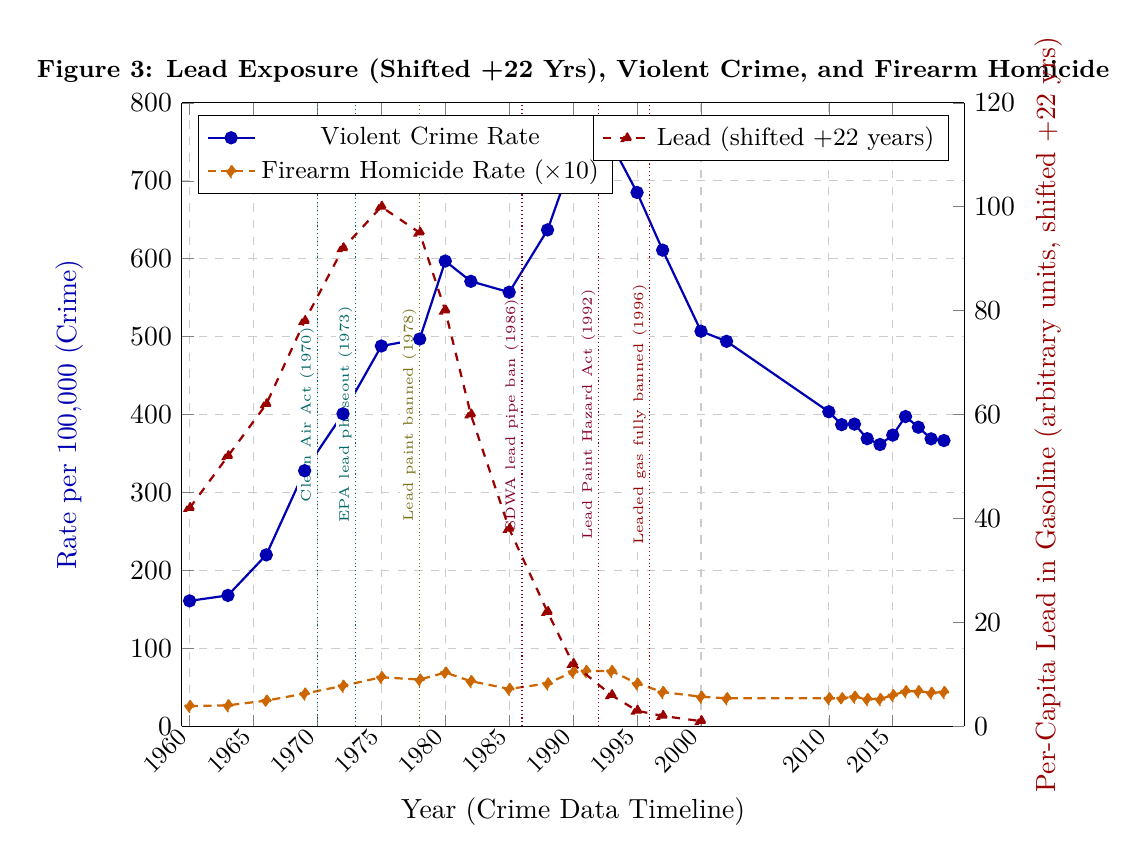
\begin{tikzpicture}
\begin{axis}[
    width=0.95\textwidth,
    height=9.5cm,
    title={\textbf{Figure 3: Lead Exposure (Shifted +22 Yrs), Violent Crime, and Firearm Homicide}},
    xlabel={Year (Crime Data Timeline)},
    ylabel={Rate per 100{,}000 (Crime)},
    axis y line*=left,
    xmin=1960, xmax=2020,
    enlarge x limits={0.04, 0.01},
    ymin=0, ymax=800,
    xtick={1960,1965,1970,1975,1980,1985,1990,1995,2000,2010,2015},
    xticklabel style={rotate=45, anchor=east, font=\small, /pgf/number format/1000 sep={}},
    grid=major,
    grid style={dashed, gray!40},
    ylabel style={blue!70!black, yshift=10pt},
    mark size=2pt,
    every axis title/.style={font=\bfseries\small, at={(0.5,1.05)}},
    legend style={at={(0.02,0.98)}, anchor=north west, font=\small},
]
\addplot[thick, blue!70!black, mark=*] coordinates {
    (1960, 161) (1963, 168) (1966, 220) (1969, 328)
    (1972, 401) (1975, 488) (1978, 497) (1980, 597)
    (1982, 571) (1985, 557) (1988, 637) (1990, 730)
    (1991, 758) (1993, 747) (1995, 685) (1997, 611)
    (2000, 507) (2002, 494)
    (2010, 403.6) (2011, 387.1) (2012, 387.8) (2013, 369.1) (2014, 361.6) (2015, 373.7) (2016, 397.5) (2017, 383.8) (2018, 368.9) (2019, 366.7)
};
\addlegendentry{Violent Crime Rate}
% Firearm homicide rate scaled x10
\addplot[thick, orange!80!black, mark=diamond*, densely dashed] coordinates {
    (1960, 26) (1963, 27) (1966, 33) (1969, 42)
    (1972, 52) (1975, 63) (1978, 60) (1980, 69)
    (1982, 58) (1985, 48) (1988, 55) (1990, 70)
    (1991, 71) (1993, 71) (1995, 55) (1997, 44)
    (2000, 38) (2002, 36)
    (2010, 36) (2011, 36) (2012, 38) (2013, 35) (2014, 35) (2015, 40) (2016, 45) (2017, 45) (2018, 43) (2019, 44)
};
\addlegendentry{Firearm Homicide Rate ($\times$10)}
% Lead policy event vertical lines with labels at mid-graph
\draw[densely dotted, teal!80!black] (axis cs:1970,0) -- (axis cs:1970,800);
\node[rotate=90, anchor=south, font=\tiny, teal!80!black, fill=white, inner sep=1pt] at (axis cs:1970,400) {Clean Air Act (1970)};
\draw[densely dotted, teal!80!black] (axis cs:1973,0) -- (axis cs:1973,800);
\node[rotate=90, anchor=south, font=\tiny, teal!80!black, fill=white, inner sep=1pt] at (axis cs:1973,400) {EPA lead phaseout (1973)};
\draw[densely dotted, olive!80!black] (axis cs:1978,0) -- (axis cs:1978,800);
\node[rotate=90, anchor=south, font=\tiny, olive!80!black, fill=white, inner sep=1pt] at (axis cs:1978,400) {Lead paint banned (1978)};
\draw[densely dotted, purple!70!black] (axis cs:1986,0) -- (axis cs:1986,800);
\node[rotate=90, anchor=south, font=\tiny, purple!70!black, fill=white, inner sep=1pt] at (axis cs:1986,400) {SDWA lead pipe ban (1986)};
\draw[densely dotted, purple!70!black] (axis cs:1992,0) -- (axis cs:1992,800);
\node[rotate=90, anchor=south, font=\tiny, purple!70!black, fill=white, inner sep=1pt] at (axis cs:1992,400) {Lead Paint Hazard Act (1992)};
\draw[densely dotted, red!60!black] (axis cs:1996,0) -- (axis cs:1996,800);
\node[rotate=90, anchor=south, font=\tiny, red!60!black, fill=white, inner sep=1pt] at (axis cs:1996,400) {Leaded gas fully banned (1996)};
\end{axis}
\begin{axis}[
    width=0.95\textwidth,
    height=9.5cm,
    axis y line*=right,
    axis x line=none,
    ylabel={Per-Capita Lead in Gasoline (arbitrary units, shifted +22 yrs)},
    xmin=1960, xmax=2020,
    enlarge x limits={0.04, 0.01},
    ymin=0, ymax=120,
    ylabel style={red!60!black},
    mark size=2pt,
    legend style={at={(0.98,0.98)}, anchor=north east, font=\small},
]
\addplot[thick, red!60!black, mark=triangle*, dashed] coordinates {
    (1960, 42) (1963, 52) (1966, 62) (1969, 78)
    (1972, 92) (1975, 100) (1978, 95) (1980, 80)
    (1982, 60) (1985, 38) (1988, 22) (1990, 12)
    (1993, 6) (1995, 3) (1997, 2) (2000, 1)
};
\addlegendentry{Lead (shifted +22 years)}
\end{axis}
\end{tikzpicture}
\caption*{\emph{Sources: Rick Nevin, ``Understanding International Crime Trends,'' Environmental Research 104 (2007); Reyes, NBER Working Paper 13097 (2007); EPA historical gasoline lead data; FBI UCR; CDC WONDER Compressed Mortality File (firearm homicide). Lead policy events: Clean Air Act (1970); EPA phaseout of tetraethyllead (1973); lead paint ban (1978); SDWA lead pipe ban (1986); Lead Paint Hazard Reduction Act (1992); total leaded gasoline prohibition (1996). Note: Lead data shifted +22 years; firearm homicide scaled $\times$10. Both the firearm homicide curve and the overall violent crime curve track the lagged lead-exposure curve with striking fidelity, declining in tandem as the detoxified generation ages into adulthood.}}
\end{figure}

\clearpage

\subsection{\texorpdfstring{\textbf{The Macro-Economic Void:
Deindustrialization and the Urban
Underclass}}{The Macro-Economic Void: Deindustrialization and the Urban Underclass}}\label{the-macro-economic-void-deindustrialization-and-the-urban-underclass}

The theoretical models of strain and social disorganization were
aggressively catalyzed by the macro-economic phenomenon of
deindustrialization. Beginning in the late 1960s and accelerating
rapidly through the 1970s and 1980s, the United States transitioned from
a manufacturing-based economy to a service-based economy, a shift that
effectively hollowed out the economic core of numerous urban centers.\\
The systemic effects of this economic restructuring are perfectly
encapsulated by the case study of Youngstown, Ohio. Over the course of
the 1980s, Youngstown lost an estimated 50,000 jobs in the steel and
related manufacturing industries. This sudden evaporation of secure,
middle-class, blue-collar employment triggered a cascading series of
social costs. The subsequent decline in the municipal tax base forced
massive mandatory cutbacks to essential public services, including
police and fire departments, sanitation, and street maintenance. The
physical decay of the city---characterized by abandoned industrial
``brownfields'' and deteriorating infrastructure---birthed a localized
``broken window syndrome'' that repelled new investment, plummeting
property values and trapping the remaining population in a downward
economic spiral.\\
Crucially, the loss of industrial employment left a generational void.
Young adults coming of age in the late 1970s and 1980s faced a
bifurcated labor market where the only available options were
low-paying, contingent service sector jobs that lacked the benefits,
union protection, and stability enjoyed by their parents. Sociologist
William Julius Wilson documented this phenomenon extensively, arguing
that the flight of manufacturing jobs, coupled with the outward
migration of the Black middle class to the suburbs, created a phenomenon
of ``spatial mismatch'' where impoverished minority populations were
left concentrated in inner cities entirely devoid of economic
opportunity.\\
Criminologists observed that as unemployment and economic insecurity
spread, localized street crime predictably escalated. Property crimes
served as an alternative economic engine, while the resulting
hopelessness and frustration manifested in violence. Research indicates
that economic restructuring between 1970 and 1990 increased homicide
rates as economic deprivation deepened. By the 1990s, heavily
deindustrialized cities like Youngstown and Gary, Indiana, exhibited
some of the highest per capita murder rates in the nation. In a
desperate bid for economic salvation, many of these hollowed-out
municipalities turned to the prison industry. Cities that had once
forged steel began aggressively courting the construction of state and
private correctional facilities, thereby transforming into ``prison
economies'' that provided low-quality security jobs while simultaneously
expanding the geographic footprint of the carceral state.

\begin{figure}[ht]
\centering
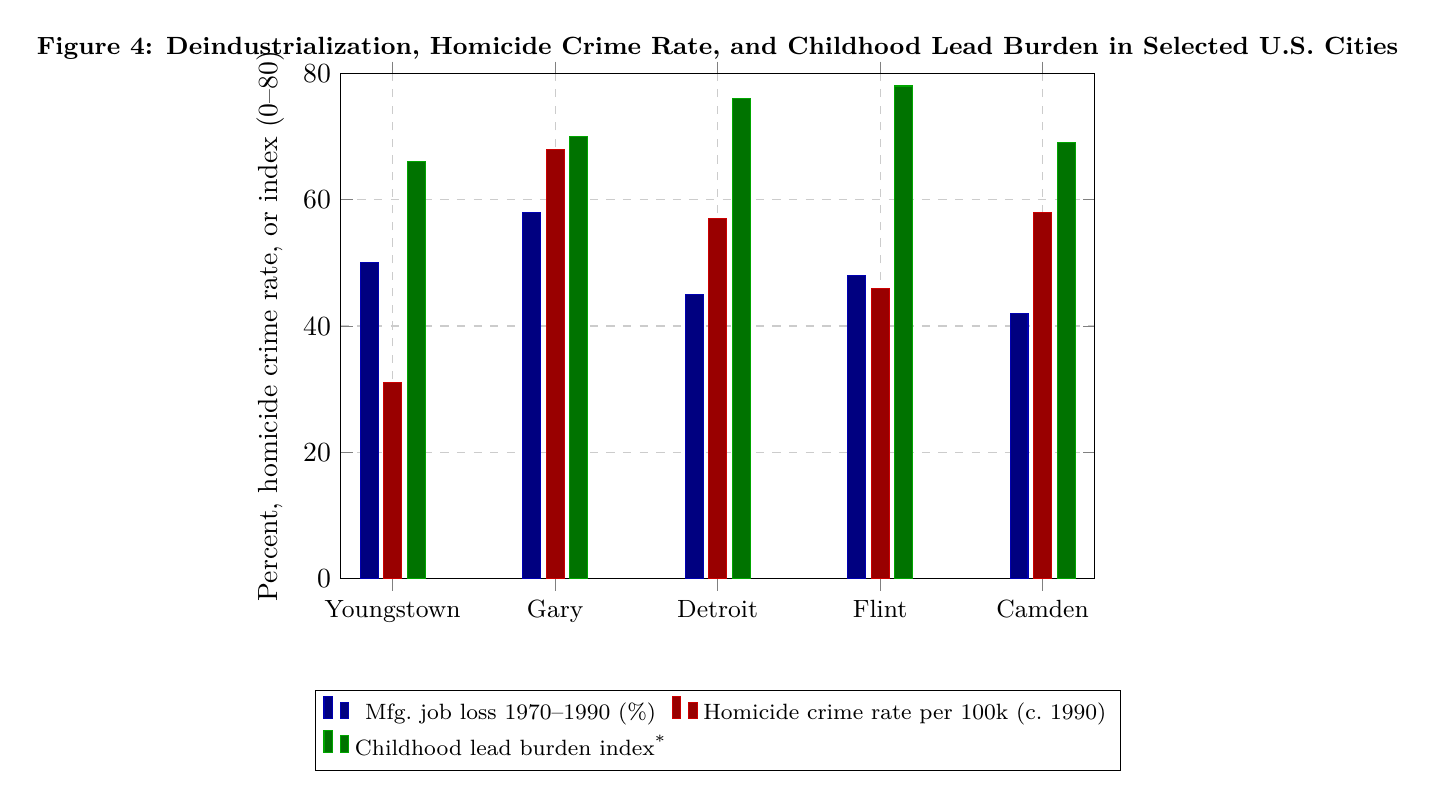
\begin{tikzpicture}
\begin{axis}[
    width=0.92\textwidth,
    height=8cm,
    title={\textbf{Figure 4: Deindustrialization, Homicide Crime Rate, and Childhood Lead Burden in Selected U.S.\ Cities}},
    ybar,
    bar width=6.5pt,
    enlarge x limits=0.08,
    ylabel={Percent, homicide crime rate, or index (0--80)},
    symbolic x coords={Youngstown, Gary, Detroit, Flint, Camden},
    xtick=data,
    xticklabel style={font=\small, /pgf/number format/1000 sep={}},
    ymin=0, ymax=80,
    grid=major,
    grid style={dashed, gray!40},
    every axis title/.style={font=\bfseries\small, at={(0.5,1.05)}},
    legend style={at={(0.5,-0.22)}, anchor=north, font=\footnotesize, legend columns=2},
]
\addplot[fill=blue!50!black, draw=blue!70!black] coordinates {
    (Youngstown, 50) (Gary, 58) (Detroit, 45) (Flint, 48) (Camden, 42)
};
\addlegendentry{Mfg.\ job loss 1970--1990 (\%)}
\addplot[fill=red!60!black, draw=red!80!black] coordinates {
    (Youngstown, 31) (Gary, 68) (Detroit, 57) (Flint, 46) (Camden, 58)
};
\addlegendentry{Homicide crime rate per 100k (c.\ 1990)}
\addplot[fill=green!45!black, draw=green!65!black] coordinates {
    (Youngstown, 66) (Gary, 70) (Detroit, 76) (Flint, 78) (Camden, 69)
};
\addlegendentry{Childhood lead burden index\textsuperscript{*}}
\end{axis}
\end{tikzpicture}
\caption*{\emph{Sources: Bureau of Labor Statistics, Current Employment Statistics (historical metro-area data); FBI UCR city-level crime data; William Julius Wilson, ``When Work Disappears: The World of the New Urban Poor'' (1996); CDC childhood lead surveillance summaries and HUD risk proxies (composite index, illustrative 0--80 scale aligned to chart for comparison). \textsuperscript{*}Lead index approximates relative elevated blood-lead prevalence among children during the 1975--1985 window in legacy industrial housing and high-traffic corridors; it is not expressed in homicide or percentage units. Cities that suffered the steepest manufacturing losses consistently registered among the nation's highest homicide crime rates by 1990 and typically carried heavy overlapping lead loads.}}
\end{figure}

\clearpage

\subsection{\texorpdfstring{\textbf{Market Catalysts: Crack Cocaine,
Firearm Proliferation, and the Youth
Bulge}}{Market Catalysts: Crack Cocaine, Firearm Proliferation, and the Youth Bulge}}\label{market-catalysts-crack-cocaine-firearm-proliferation-and-the-youth-bulge}

If deindustrialization provided the economic void and lead exposure
provided the neurobiological susceptibility, the crack cocaine epidemic
of the mid-1980s provided the immediate market catalyst for lethal
violence.\\
Following the introduction of crack cocaine in the 1980s, the drug
quickly saturated impoverished urban neighborhoods. Unlike powder
cocaine, which was expensive and associated with affluent consumers,
crack was synthesized to be highly addictive, produced a brief but
intense euphoria, and was sold in inexpensive, single-dose increments.
This retail model resulted in an explosive proliferation of open-air
drug markets. In the absence of legitimate employment due to the
aforementioned deindustrialization, the illicit drug trade became one of
the few lucrative economic engines available to young, disenfranchised
urban men.\\
However, because participants in illicit markets cannot rely on the
state for dispute resolution, contract enforcement, or protection from
theft, violence became the primary mechanism for regulating the market.
Economists and sociologists note that the severe spike in youth homicide
rates in the 1980s was intimately tied to the territorial defense of
crack markets. Between 1984 and 1994, the homicide rate for Black males
aged 14 to 17 more than doubled, and the rate for those aged 18 to 24
increased nearly as much. Interestingly, the homicide rate for older
demographics remained essentially flat during this period, indicating
that the violence was hyper-concentrated in the youth demographic
actively participating in the street-level drug trade.\\
Simultaneously, this period witnessed a massive ``supply shock'' in the
production and distribution of cheap, easily concealable handguns. Prior
to the 1980s, youth gang conflicts were largely mediated by physical
altercations or blunt weapons like brass knuckles. The sudden influx of
firearms into urban environments transformed localized, non-fatal
disputes into lethal encounters. Gangs shifted from territorial social
groups into highly armed, entrepreneurial drug-trafficking
organizations. The symbiotic relationship between the lucrative crack
trade and the widespread availability of high-capacity firearms acted as
a profound force multiplier, pushing the national homicide rate to its
1991 peak.\\
The severity of this market-driven violence intersected with demographic
realities. Criminologists analyze cohort effects using age-period-cohort
(APC) models, which demonstrate that crime is heavily concentrated in
the youth demographic. During the 1980s, the United States experienced a
localized ``youth bulge''---a demographic anomaly where an unusually
large proportion of the population entered the high-risk ages of 15 to
24 simultaneously. Political scientists like Gunnar Heinsohn and Gary
Fuller have documented that when a rapidly growing youth population
intersects with weak institutional control and resource scarcity, the
risk of political violence and violent crime increases exponentially.\\
In the US context, this youth bulge collided directly with the economic
devastation of deindustrialization and the allure of the crack cocaine
trade. This demographic reality temporarily blinded researchers;
prominent social scientists in the early 1990s notoriously predicted an
impending wave of juvenile ``super-predators''---a generation of
violently remorseless youth that would ravage the country by the year
2000. This deterministic demographic hypothesis proved disastrously
incorrect, as juvenile crime plummeted shortly after 1994, but the
immense fear generated by this rhetoric heavily influenced the punitive
policy responses of the era.

\begin{figure}[ht]
\centering
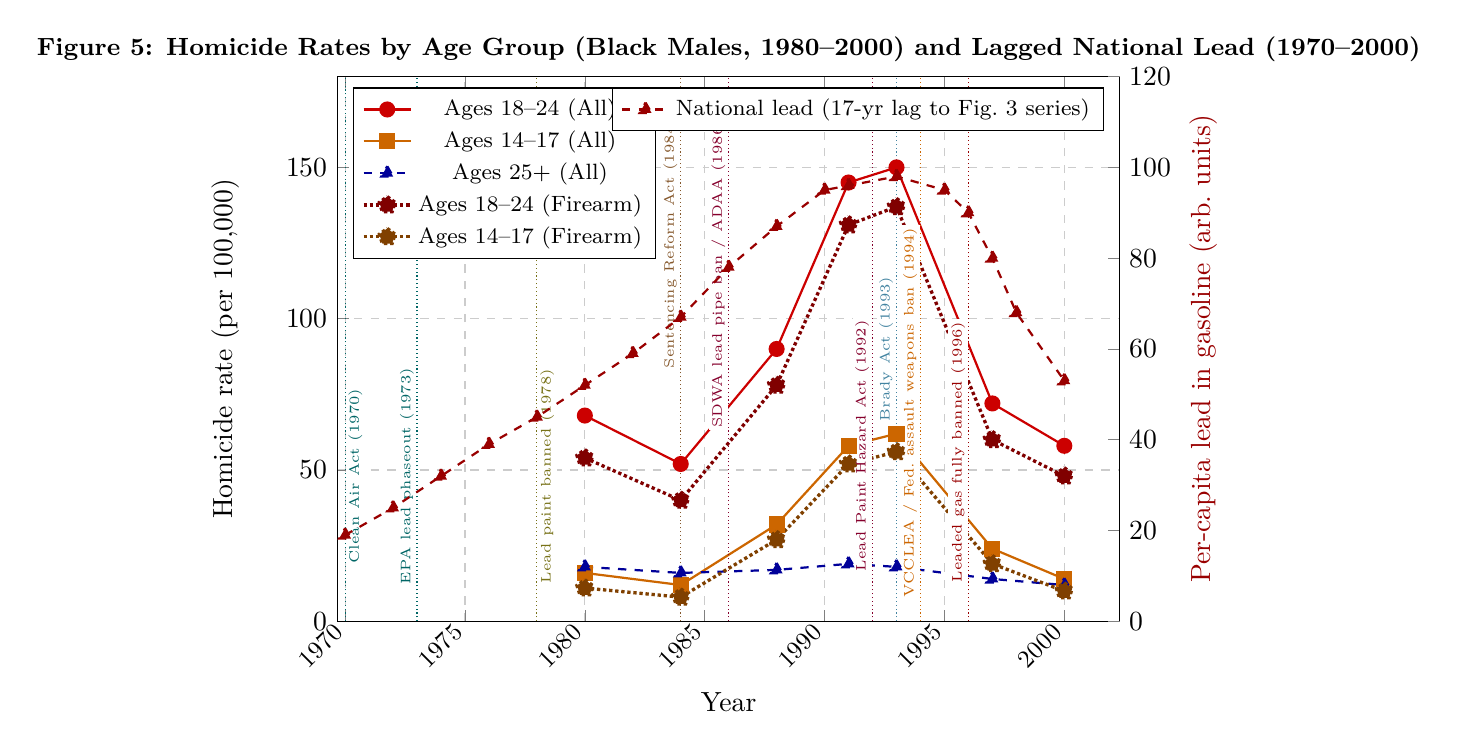
\begin{tikzpicture}
\begin{axis}[
    width=0.95\textwidth,
    height=8.5cm,
    title={\textbf{Figure 5: Homicide Rates by Age Group (Black Males, 1980--2000) and Lagged National Lead (1970--2000)}},
    xlabel={Year},
    ylabel={Homicide rate (per 100{,}000)},
    axis y line*=left,
    xmin=1970, xmax=2002,
    enlarge x limits={0.04, 0.01},
    ymin=0, ymax=180,
    xtick={1970,1975,1980,1985,1990,1995,2000},
    xticklabel style={rotate=45, anchor=east, font=\small, /pgf/number format/1000 sep={}},
    grid=major,
    grid style={dashed, gray!40},
    ylabel style={yshift=10pt},
    mark size=2.5pt,
    every axis title/.style={font=\bfseries\small, at={(0.5,1.05)}},
    legend style={at={(0.02,0.98)}, anchor=north west, font=\footnotesize},
]
% Total homicide by age group
\addplot[thick, red!80!black, mark=*] coordinates {
    (1980, 68) (1984, 52) (1988, 90) (1991, 145) (1993, 150) (1997, 72) (2000, 58)
};
\addlegendentry{Ages 18--24 (All)}
\addplot[thick, orange!80!black, mark=square*] coordinates {
    (1980, 16) (1984, 12) (1988, 32) (1991, 58) (1993, 62) (1997, 24) (2000, 14)
};
\addlegendentry{Ages 14--17 (All)}
\addplot[thick, blue!60!black, mark=triangle*, dashed] coordinates {
    (1980, 18) (1984, 16) (1988, 17) (1991, 19) (1993, 18) (1997, 14) (2000, 12)
};
\addlegendentry{Ages 25+ (All)}
% Firearm-specific homicide for 18-24 cohort
\addplot[very thick, red!50!black, mark=pentagon*, densely dotted, mark size=3pt] coordinates {
    (1980, 54) (1984, 40) (1988, 78) (1991, 131) (1993, 137) (1997, 60) (2000, 48)
};
\addlegendentry{Ages 18--24 (Firearm)}
% Firearm-specific homicide for 14-17 cohort
\addplot[very thick, orange!50!black, mark=pentagon*, densely dotted, mark size=3pt] coordinates {
    (1980, 11) (1984, 8) (1988, 27) (1991, 52) (1993, 56) (1997, 19) (2000, 10)
};
\addlegendentry{Ages 14--17 (Firearm)}
% --- Policy markers (lead: Figure 3 style; crime/gun: Figures 1--2) ---
\draw[densely dotted, teal!80!black] (axis cs:1970,0) -- (axis cs:1970,180);
\node[rotate=90, anchor=north, font=\tiny, teal!80!black, fill=white, inner sep=1pt] at (axis cs:1970,48) {Clean Air Act (1970)};
\draw[densely dotted, teal!80!black] (axis cs:1973,0) -- (axis cs:1973,180);
\node[rotate=90, anchor=south, font=\tiny, teal!80!black, fill=white, inner sep=1pt] at (axis cs:1973,48) {EPA lead phaseout (1973)};
\draw[densely dotted, olive!80!black] (axis cs:1978,0) -- (axis cs:1978,180);
\node[rotate=90, anchor=north, font=\tiny, olive!80!black, fill=white, inner sep=1pt] at (axis cs:1978,48) {Lead paint banned (1978)};
\draw[densely dotted, purple!70!black] (axis cs:1986,0) -- (axis cs:1986,180);
\node[rotate=90, anchor=south, font=\tiny, purple!70!black, fill=white, inner sep=1pt] at (axis cs:1986,115) {SDWA lead pipe ban / ADAA (1986)};
\draw[densely dotted, brown!70!black] (axis cs:1984,0) -- (axis cs:1984,180);
\node[rotate=90, anchor=south, font=\tiny, brown!70!black, fill=white, inner sep=1pt] at (axis cs:1984,125) {Sentencing Reform Act (1984)};
\draw[densely dotted, cyan!60!black] (axis cs:1993,0) -- (axis cs:1993,180);
\node[rotate=90, anchor=south, font=\tiny, cyan!60!black, fill=white, inner sep=1pt] at (axis cs:1993,90) {Brady Act (1993)};
\draw[densely dotted, purple!70!black] (axis cs:1992,0) -- (axis cs:1992,180);
\node[rotate=90, anchor=south, font=\tiny, purple!70!black, fill=white, inner sep=1pt] at (axis cs:1992,58) {Lead Paint Hazard Act (1992)};
\draw[densely dotted, orange!80!black] (axis cs:1994,0) -- (axis cs:1994,180);
\node[rotate=90, anchor=south, font=\tiny, orange!80!black, fill=white, inner sep=1pt] at (axis cs:1994,69) {VCCLEA / Fed.\ assault weapons ban (1994)};
\draw[densely dotted, red!60!black] (axis cs:1996,0) -- (axis cs:1996,180);
\node[rotate=90, anchor=south, font=\tiny, red!60!black, fill=white, inner sep=1pt] at (axis cs:1996,56) {Leaded gas fully banned (1996)};
\end{axis}
\begin{axis}[
    width=0.95\textwidth,
    height=8.5cm,
    axis y line*=right,
    axis x line=none,
    xmin=1970, xmax=2002,
    enlarge x limits={0.04, 0.01},
    ymin=0, ymax=120,
    ylabel={Per-capita lead in gasoline (arb.\ units)},
    ylabel style={red!60!black},
    mark size=2.5pt,
    legend style={at={(0.98,0.98)}, anchor=north east, font=\footnotesize},
]
% National gasoline lead: at plot year $Y$, value matches Figure~3 lead at $x=Y-17$. For $Y<1977$, $x<1960$: linear extrapolation from first Fig.~3 segment (1960--1963). Else interpolate between Fig.~3 anchors. Shorter lag than Fig.~3's +22 so late-1990s youth cohorts map to early-1980s declining ambient lead.
\addplot[thick, red!60!black, mark=triangle*, dashed] coordinates {
    (1970, 19) (1972, 25) (1974, 32) (1976, 39) (1978, 45)
    (1980, 52) (1982, 59) (1984, 67) (1986, 78) (1988, 87) (1990, 95)
    (1991, 96) (1993, 98) (1995, 95) (1996, 90) (1997, 80) (1998, 68) (2000, 53)
};
\addlegendentry{National lead (17-yr lag to Fig.\ 3 series)}
\end{axis}
\end{tikzpicture}
\caption*{\emph{Sources: BJS, ``Homicide Trends in the United States, 1980--2008''; Urban Institute, ``The Rise and Fall of American Youth Violence: 1980 to 2000''; CDC WONDER Compressed Mortality File (firearm-specific); Rick Nevin, ``Understanding International Crime Trends,'' \emph{Environmental Research} 104 (2007); EPA historical gasoline lead data. Vertical markers follow Figure 3 (lead) and Figures 1--2 (sentencing, Brady, 1994 crime bill / assault weapons ban). Right axis: same national gasoline-lead profile as Figure 3, indexed with a \textbf{17-year} offset (plot year $t$ maps to Figure~3 anchor $x=t-17$) so each year aligns with approximate early-childhood exposure for cohorts entering peak young-adult ages---avoiding the counterintuitive flat tail from a 22-year map (e.g.\ 1997$\to$1975 still near peak gasoline lead). The lead trace runs from \textbf{1970}; for $t<1977$, $x<1960$, so those values \textbf{extrapolate} linearly from the earliest Figure~3 segment (1960--1963) until pre-1960 EPA/Nevin anchors are digitized; for later years, \textbf{interpolate} between Figure~3 anchors. Homicide series (left axis) remain from 1980 per the homicide sources. Not Black-male-specific BLL. Firearm homicides (dotted) dominated youth homicide in the crack era; ages 25+ stayed flat.}}
\end{figure}

\#\# The Mathematics of Systemic Racism and Spatial Disadvantage\\
To fully comprehend the localized intensity of the crime surge, it is
necessary to examine the historical architecture of spatial
disadvantage. The crime wave did not affect all American communities
equally; it was heavily concentrated in neighborhoods subjected to
generations of state-sponsored systemic racism, most notably through the
practice of redlining.\\
In the 1930s, the Home Owners' Loan Corporation (HOLC) created
residential security maps that graded neighborhoods from A (Green/Best)
to D (Red/Hazardous) based heavily on their racial and ethnic
composition. Neighborhoods with Black, immigrant, or mixed populations
were systematically ``redlined,'' entirely cutting them off from federal
mortgage backing and private capital. This state-mandated disinvestment
locked these communities out of the primary mechanism of American wealth
generation: homeownership. Over the subsequent decades, these redlined
areas devolved into zones of concentrated poverty, deteriorating
housing, and failing infrastructure.\\
Modern geospatial analysis reveals a near-perfect spatial correlation
between the HOLC redlining maps of the 1930s and the intense clusters of
firearm homicides, violent crime, and lead poisoning in the 1980s and
1990s. Due to the deterioration of housing stock and proximity to
industrial corridors, residents in redlined zones absorbed vastly
disproportionate amounts of environmental lead, biologically
handicapping the youth population before they even reached
adolescence.\\
Recent sociological scholarship has sought to quantify this systemic
oppression through mathematical set theory, revealing critical insights
into the nature of the crime surge. Traditional analyses often model
systemic disadvantage using simple summation
(\textbackslash Sigma)---suggesting that the harms of various
discriminatory policies are simply added together, and that if a policy
is repealed, the harm simply plateaus.\\
However, mathematical critiques of systemic racism argue that this
additive model is deeply flawed. Oppression functions through
non-linear, compounding harm that is best represented by \emph{iterative
functions} incorporating a temporal variable (t). A policy must be
viewed as a mathematical operation that fundamentally alters the
baseline capacity of a specific demographic set before the next policy
is applied.\\
To accurately model this historically, generic mathematical nomenclature
mapping an In-group (I) and Out-group (O) is insufficient and dilutes
the thesis, as it could apply to trivial group conflicts. Instead,
utilizing specific sets---such as
O\_\{\textbackslash text\{racialized\}\} or
O\_\{\textbackslash text\{African diaspora\}\}---aligns the mathematics
with the specific historical project of racial engineering. The
historical enslavement of African Americans severely reduced the
baseline capital, social standing, and political power of
O\_\{\textbackslash text\{racialized\}\}. When a subsequent policy like
redlining (P\_2) was enacted in the 1930s, its destructive impact was
exponentially magnified because it was applied to a group already
mathematically diminished by previous systemic extractions.\\
By the 1980s, when the crack epidemic and deindustrialization hit, these
geographically isolated and economically starved communities possessed
virtually zero institutional buffer. Thus, the intense localized
violence of the late 20th century was not a spontaneous cultural failure
or an inherent racial attribute, but rather the mathematically
predictable, compounding output of centuries of targeted capital
starvation and spatial engineering. A rigorous set-theory analysis
forces the conclusion that systemic racism dictates specific systemic
interventions targeting the intersection of the out-group and the policy
(O \textbackslash cap P), rather than relying on individual-focused
solutions like sensitivity training.

\begin{figure}[ht]
\centering
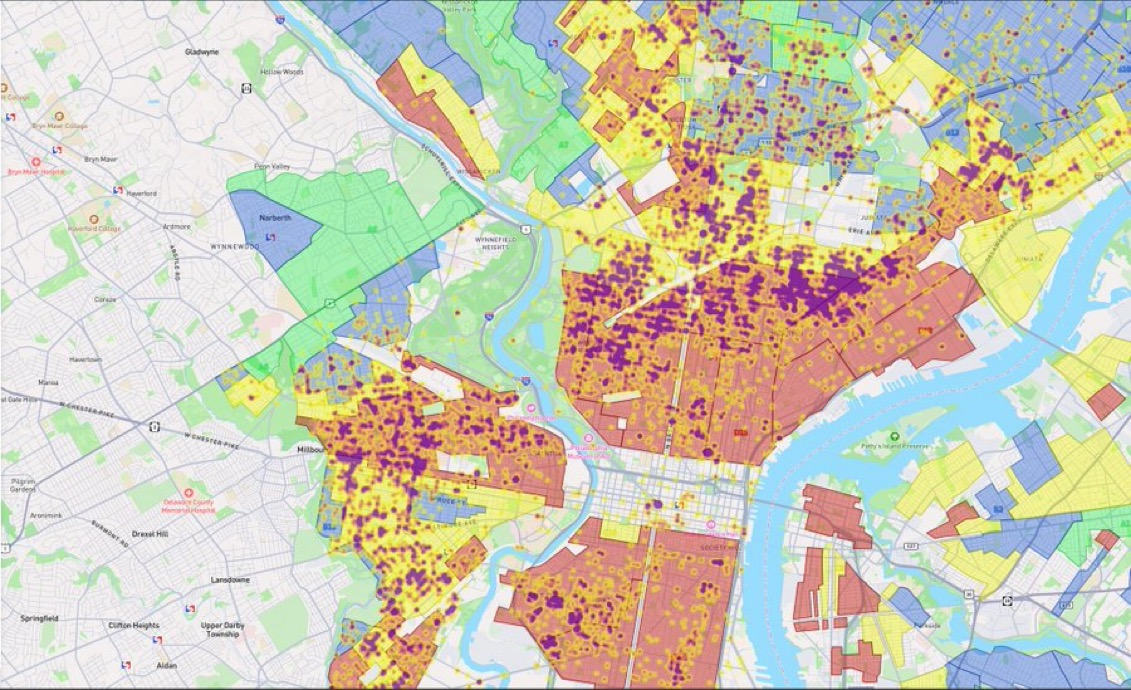
\includegraphics[width=0.95\textwidth]{Philadelphia_gun_red.jpeg}
\caption*{\textbf{Figure 6: HOLC Redlining Grades (1930s) Overlaid with Firearm Homicide Density --- Philadelphia, PA}\\[0.3cm]
\emph{HOLC residential security grades are displayed as colored zones: Grade A (green/``Best''), Grade B (blue/``Still Desirable''), Grade C (yellow/``Definitely Declining''), and Grade D (red/``Hazardous''). Firearm homicide incidents are overlaid as purple/orange density clusters. The spatial coincidence between Grade D (red) zones and the highest-density homicide clusters demonstrates the six-decade pipeline from state-mandated disinvestment to concentrated lethal violence. Areas graded A and B---which received preferential mortgage access and capital investment---show negligible homicide density. Sources: University of Richmond Digital Scholarship Lab, \emph{Mapping Inequality: Redlining in New Deal America} (HOLC grades); OpenDataPhilly, Philadelphia Police Department incident data (firearm homicides). See also: Testa et al., ``Historical Redlining and Contemporary Violent Victimization,'' PMC (2024); Jacoby et al., ``Historical Redlining and the Epidemiology of Present-Day Firearm Violence,'' PMC (2023).}}
\end{figure}

\subsection{\texorpdfstring{\textbf{Historical Antecedents of the
Carceral
Apparatus}}{Historical Antecedents of the Carceral Apparatus}}\label{historical-antecedents-of-the-carceral-apparatus}

When the crime surge of the 1970s and 1980s demanded a political
response, the state relied upon a carceral apparatus that had been
shaped by centuries of racial and economic extraction. The modern
American penal system evolved from two distinct historical kernels, both
of which laid the groundwork for the era of mass incarceration.\\
In the North, the prison system was born out of Quaker-influenced
Enlightenment reforms. Following the American Revolution, reformers like
Dr.~Benjamin Rush established the Philadelphia Society for Alleviating
the Miseries of Public Prisons, seeking a humane alternative to the
corporal and capital punishments of the colonial era. This led to the
creation of the Walnut Street Jail in 1790, and eventually the Eastern
State Penitentiary in 1829. These institutions pioneered the
``Pennsylvania System''---a model of strict, total solitary confinement
combined with labor. The theoretical goal was to isolate the individual
from corrupting social influences, allowing them to reflect on their
crimes and achieve spiritual ``penitence'' (hence, penitentiary). While
philosophically high-minded and initially viewed as a triumph of liberal
reform, this architectural model quickly devolved into profound
psychological torture and rigid institutional control, establishing the
precedent that the state possessed the absolute authority to warehouse
and isolate human bodies.\\
Conversely, the Southern penal system evolved as a direct continuation
of racial subjugation and economic exploitation following the Civil War.
The ratification of the 13th Amendment in 1865 abolished chattel
slavery, but it contained a critical, deliberate loophole: ``Neither
slavery nor involuntary servitude, \emph{except as a punishment for
crime} whereof the party shall have been duly convicted, shall exist
within the United States''.\\
This clause facilitated a massive \emph{interface shift} in the
machinery of oppression. White supremacist regimes across the South
quickly enacted ``Black Codes''---strict, highly subjective misdemeanor
laws criminalizing vagrancy, loitering, walking on grass, or lacking
proof of employment. These laws were applied in a racially
discriminatory manner to arbitrarily arrest tens of thousands of newly
freed Black citizens. Once convicted, these individuals were leased out
to private corporations, coal mines, lumber yards, and plantations under
the brutal ``convict leasing'' system.\\
This system generated massive revenue; by 1898, convict leasing
accounted for 73\% of the state of Alabama's revenue. Major national
corporations, such as the Tennessee Coal, Iron, and Railroad Company
(later part of U.S. Steel), extracted vast wealth from this captive
labor force, subjecting prisoners to lethal working conditions with zero
accountability for their survival. Therefore, the foundational
``kernel'' of the American justice system was inextricably linked to
private profit, the commodification of captive bodies, and racial
control. When urban crime rates spiked a century later, the structural,
legal, and ideological frameworks to warehouse and extract value from
marginalized populations were already deeply entrenched.

\subsection{\texorpdfstring{\textbf{Legislative Architecture: The War on
Drugs and Broken
Windows}}{Legislative Architecture: The War on Drugs and Broken Windows}}\label{legislative-architecture-the-war-on-drugs-and-broken-windows}

Faced with rising crime, profound public anxiety, and a highly mobilized
electorate, politicians in the late 20th century aggressively weaponized
this historical carceral apparatus, initiating the modern era of mass
incarceration.\\
The primary vehicle for this expansion was the ``War on Drugs.''
Initially declared by President Richard Nixon in 1971, the campaign
named drug abuse as ``public enemy number one,'' framing addiction
entirely as a criminal and moral failure rather than a public health
crisis. The underlying motivations for this policy were explicitly
political and racial. In a later interview, Nixon's domestic policy
chief, John Ehrlichman, bluntly admitted that the administration
intentionally criminalized marijuana and heroin to disrupt, vilify, and
incarcerate their two primary political enemies: the anti-war left and
Black communities.\\
The drug war escalated dramatically under President Ronald Reagan in the
1980s. Driven by intense media coverage of the crack epidemic and
catalyzed by the highly publicized 1986 cocaine-induced death of
basketball star Len Bias, Congress passed the Anti-Drug Abuse Act of
1986. This legislation allocated \$1.7 billion to the drug war and
established draconian mandatory minimum sentences that stripped judges
of their discretionary power.\\
Crucially, the law codified an egregious 100-to-1 sentencing disparity
between crack cocaine (predominantly associated with impoverished Black
communities) and powder cocaine (associated with affluent White
communities). Consequently, an individual possessing just five grams of
crack received the same automatic five-year prison sentence as someone
possessing 500 grams of powder cocaine. This disparity acted as a
devastating \emph{interface shift} in systemic racism; it effectively
utilized proxy variables (drug type) to target and incarcerate massive
swaths of the minority Out-group while maintaining the façade of
race-neutral legality. Between 1980 and 1997, the number of individuals
incarcerated in the United States skyrocketed from 329,000 to over 1.2
million, heavily driven by nonviolent drug offenses.\\
Simultaneously, local law enforcement agencies underwent a profound
philosophical shift by adopting ``Broken Windows'' policing. Based on a
1982 sociological theory by George L. Kelling and James Q. Wilson, this
strategy posited that ignoring minor, visible signs of physical and
social disorder (like broken windows, vandalism, fare evasion, or
vagrancy) signaled a lack of community control, thereby emboldening
violent criminals to operate in those spaces.\\
In practice, particularly under New York Mayor Rudolph Giuliani and
Police Commissioner Bill Bratton in the 1990s, this theory evolved into
aggressive ``zero-tolerance'' policing. Police departments heavily
prioritized the enforcement of low-level misdemeanors, resulting in the
disproportionate harassment, stopping, frisking, and arresting of Black
and Hispanic youth. While proponents credited this strategy with
salvaging neighborhoods and driving down violent crime, critical
sociological analysis and subsequent empirical research suggest a
different reality. The strategy alienated vulnerable communities, eroded
public trust in law enforcement, and funneled millions into the criminal
justice system for trivial offenses. Furthermore, evidence suggests that
the actual crime decline was driven by broader macro-economic and
demographic trends, rather than the mass arrest of turnstile jumpers.

\begin{figure}[ht]
\centering
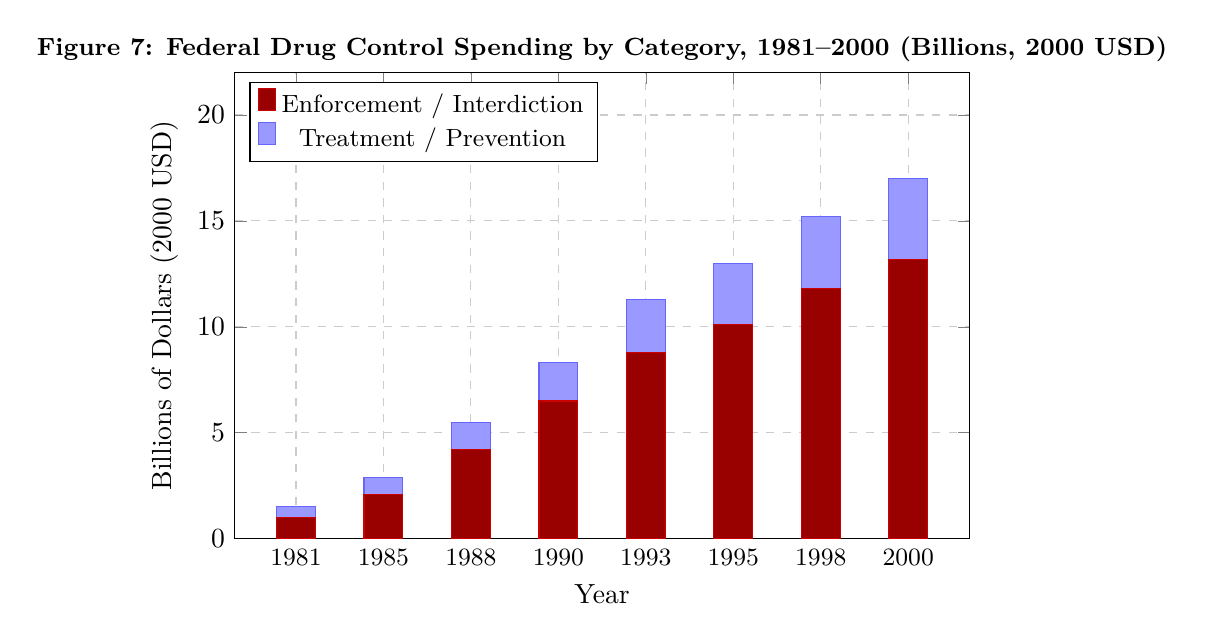
\begin{tikzpicture}
\begin{axis}[
    width=0.9\textwidth,
    height=7.5cm,
    title={\textbf{Figure 7: Federal Drug Control Spending by Category, 1981--2000 (Billions, 2000 USD)}},
    ybar stacked,
    bar width=14pt,
    xlabel={Year},
    ylabel={Billions of Dollars (2000 USD)},
    symbolic x coords={1981,1985,1988,1990,1993,1995,1998,2000},
    xtick=data,
    xticklabel style={font=\small, /pgf/number format/1000 sep={}},
    ymin=0, ymax=22,
    grid=major,
    grid style={dashed, gray!40},
    every axis title/.style={font=\bfseries\small, at={(0.5,1.05)}},
    legend style={at={(0.02,0.98)}, anchor=north west, font=\small},
]
\addplot[fill=red!60!black, draw=red!80!black] coordinates {
    (1981, 1.0) (1985, 2.1) (1988, 4.2) (1990, 6.5)
    (1993, 8.8) (1995, 10.1) (1998, 11.8) (2000, 13.2)
};
\addlegendentry{Enforcement / Interdiction}
\addplot[fill=blue!40, draw=blue!60] coordinates {
    (1981, 0.5) (1985, 0.8) (1988, 1.3) (1990, 1.8)
    (1993, 2.5) (1995, 2.9) (1998, 3.4) (2000, 3.8)
};
\addlegendentry{Treatment / Prevention}
\end{axis}
\end{tikzpicture}
\caption*{\emph{Sources: Office of National Drug Control Policy (ONDCP), National Drug Control Budget summaries (annual); Drug Policy Alliance, historical spending compilations; Jonathan Caulkins et al., ``How Goes the `War on Drugs'?'' RAND Corporation (2005). Note: Enforcement and interdiction consistently consumed approximately 65--75\% of federal drug control spending, while treatment and prevention were chronically underfunded---even as Black civic leaders specifically requested comprehensive public health investment.}}
\end{figure}

\begin{figure}[ht]
\centering
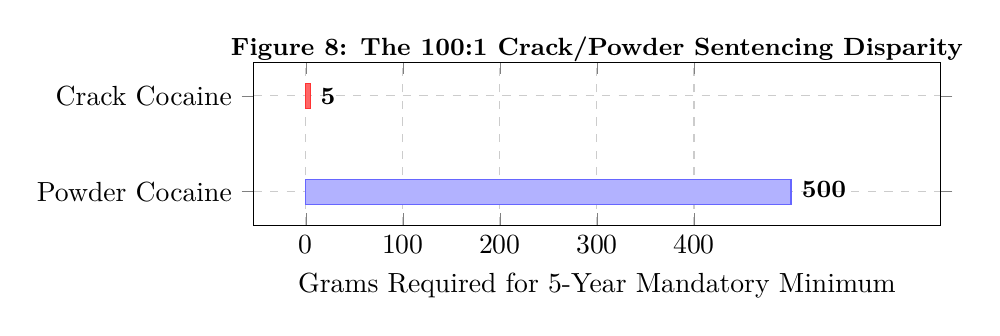
\begin{tikzpicture}
\begin{axis}[
    width=0.85\textwidth,
    height=3.65cm,
    title={\textbf{Figure 8: The 100:1 Crack/Powder Sentencing Disparity}},
    xbar,
    bar width=9pt,
    bar shift=0pt,
    enlarge y limits={abs=0.35},
    xlabel={Grams Required for 5-Year Mandatory Minimum},
    ytick={0,1},
    yticklabels={Powder Cocaine, Crack Cocaine},
    yticklabel style={font=\normalsize},
    xticklabel style={/pgf/number format/1000 sep={}},
    xmin=0, xmax=600,
    enlarge x limits={0, 0.09},
    xtick={0,100,200,300,400},
    grid=major,
    grid style={dashed, gray!40},
    every axis title/.style={font=\bfseries\small, at={(0.5,1.08)}},
    clip=false,
]
\addplot[fill=blue!30, draw=blue!60] coordinates {(500,0)};
\addplot[fill=red!60, draw=red!80] coordinates {(5,1)};
\node[font=\small\bfseries, anchor=mid west, inner sep=2pt] at (axis cs:505,0) {500};
\node[font=\small\bfseries, anchor=mid west, inner sep=2pt, yshift=-0.8pt] at (axis cs:9,1) {5};
\end{axis}
\end{tikzpicture}

\vspace{0.3cm}
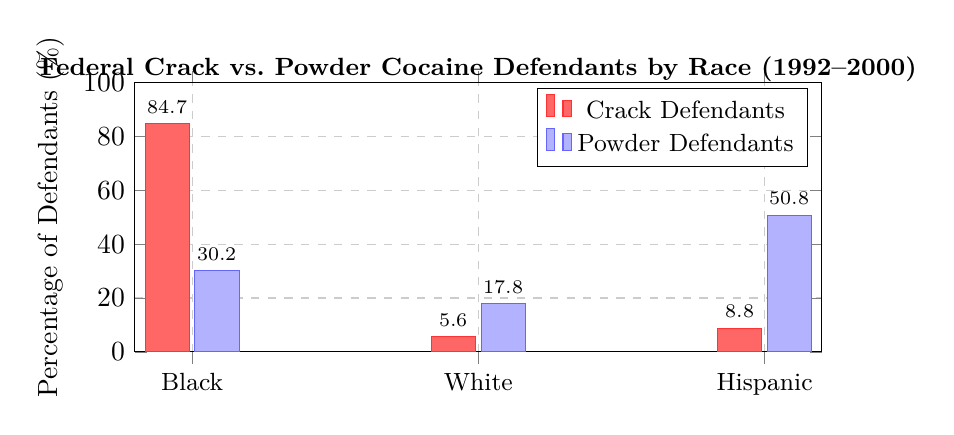
\begin{tikzpicture}
\begin{axis}[
    width=0.85\textwidth,
    height=5cm,
    title={\textbf{Federal Crack vs.\ Powder Cocaine Defendants by Race (1992--2000)}},
    ybar,
    bar width=16pt,
    ylabel={Percentage of Defendants (\%)},
    symbolic x coords={Black, White, Hispanic},
    xtick=data,
    xticklabel style={font=\small, /pgf/number format/1000 sep={}},
    ymin=0, ymax=100,
    grid=major,
    grid style={dashed, gray!40},
    every axis title/.style={font=\bfseries\small, at={(0.5,1.05)}},
    legend style={at={(0.98,0.98)}, anchor=north east, font=\small},
    nodes near coords,
    nodes near coords style={font=\scriptsize},
]
\addplot[fill=red!60, draw=red!80] coordinates {
    (Black, 84.7) (White, 5.6) (Hispanic, 8.8)
};
\addlegendentry{Crack Defendants}
\addplot[fill=blue!30, draw=blue!60] coordinates {
    (Black, 30.2) (White, 17.8) (Hispanic, 50.8)
};
\addlegendentry{Powder Defendants}
\end{axis}
\end{tikzpicture}
\caption*{\emph{Sources: U.S.\ Sentencing Commission, ``Special Report to Congress: Cocaine and Federal Sentencing Policy'' (1995, 2002 editions); Anti-Drug Abuse Act of 1986. Note: The 100:1 weight disparity meant that 5 grams of crack triggered the same mandatory minimum as 500 grams of powder cocaine. Because 85\% of federal crack defendants were Black---while powder cocaine prosecutions skewed heavily Hispanic and White---the statute functioned as a racial proxy, achieving racially discriminatory mass incarceration under the fa\c{c}ade of race-neutral legislation.}}
\end{figure}

\subsection{\texorpdfstring{\textbf{Asymmetric Choice: Black Leadership
and the 1994 Crime
Bill}}{Asymmetric Choice: Black Leadership and the 1994 Crime Bill}}\label{asymmetric-choice-black-leadership-and-the-1994-crime-bill}

The political culmination of the tough-on-crime era was the Violent
Crime Control and Law Enforcement Act of 1994. Authored primarily by
Senator Joe Biden and championed by President Bill Clinton, the 350-page
bill was the most sweeping crime legislation in U.S. history. Intended
to demonstrate that the Democratic Party could outflank Republicans on
law and order, the bill authorized \$9 billion for prison construction,
funded the hiring of 100,000 new police officers (the COPS program),
expanded the federal death penalty to 60 new offenses, and instituted
harsh ``three-strikes'' mandatory life sentences.\\
While the 1994 Crime Bill is heavily criticized today for providing the
federal funding and financial incentives that locked mass incarceration
into place for another decade , analyzing the legislation through a
historical frameworks lens requires grappling with the complex, painful
reality of Black political support at the time.\\
In his Pulitzer Prize-winning book \emph{Locking Up Our Own: Crime and
Punishment in Black America}, legal scholar James Forman Jr.~explores
the agonizing choices faced by African American civic leaders, mayors,
and the Congressional Black Caucus (CBC) during the height of the
crisis. In the late 1980s and early 1990s, Black communities were
bearing the absolute brunt of the lethal violence spawned by the crack
epidemic and the handgun supply shock. Forman notes that at the time,
Black leaders frequently compared crack cocaine to the ``greatest evils
that African Americans had ever suffered''.\\
Faced with a terrifying mortality rate among young Black men, community
residents demanded immediate state protection. Harvard law professor
Randall Kennedy observed that historically, Black Americans suffered
profoundly from being ``left unprotected or under-protected by law
enforcement''. As a result, 58\% of African Americans surveyed by Gallup
in 1994 supported the Crime Bill, compared to 49\% of White Americans,
and a delegation of Black mayors actively lobbied Congress for its
passage. Representative James Clyburn recalled that constituents viewed
crack as a ``scourge'' and demanded the government get tough to remove
it from their neighborhoods.\\
However, this support was born of an \emph{asymmetric choice} paradigm.
Black leaders, including the CBC, fundamentally recognized the systemic,
economic roots of the violence. They actively lobbied for holistic,
comprehensive investments: an ``all-of-the-above'' approach that
included substantial funding for drug treatment, job creation,
educational infrastructure, and community housing, in addition to better
policing. They introduced alternative bills emphasizing prevention and
fiercely opposed the punitive elements of the legislation, such as the
mandatory minimums and the revocation of Pell Grants for incarcerated
individuals.\\
Despite these efforts, the political machinery of the 1990s offered a
devastating ultimatum. The state was entirely willing to fund police
expansion and prison construction, but steadfastly refused to adequately
fund the requested social and economic infrastructure, deriding
prevention programs as ``pork''. Desperate to staunch the bleeding in
their neighborhoods, and presented with a binary choice between punitive
state intervention or continued lethal anarchy, a majority of the CBC
ultimately compromised and voted for the bill, securing minor
concessions like the Violence Against Women Act and the Assault Weapons
Ban.\\
The tragedy, as Forman and others analyze, is that this coerced reliance
on the carceral state severely deepened the crisis. The bill exacerbated
racial disparities, fueled aggressive over-policing, and funneled a
generation of young minority men into a penal system rooted in historic
extraction.

\subsection{\texorpdfstring{\textbf{Retrospective Diagnostics:
Deciphering the Great Crime
Decline}}{Retrospective Diagnostics: Deciphering the Great Crime Decline}}\label{retrospective-diagnostics-deciphering-the-great-crime-decline}

In a profound historical paradox, almost immediately following the
passage of the draconian 1994 Crime Bill, violent crime rates in the
United States began a precipitous, unpredicted, and sustained decline
that lasted well into the 21st century. By 2000, the violent crime rate
had dropped drastically, and it continued to fall until it reached
historic lows not seen since the 1960s.\\
Criminologists, economists, and sociologists have spent decades
attempting to isolate the causes of this ``Great Crime Decline.'' The
academic consensus firmly rejects the notion that zero-tolerance
policing or extreme incarceration alone solved the crisis. In fact,
comprehensive assessments, such as those by the National Research
Council and the Brennan Center for Justice, indicate that the
crime-reduction benefits of mass incarceration reached a point of
rapidly diminishing returns by the 1990s, and its effect on crime rates
since 2000 has been essentially non-existent. Imprisonment severely
reduced the lifetime earnings potential of offenders, disrupting
families and ultimately contributing to localized crime problems upon
their release.\\
In a seminal 2004 econometric analysis, Steven D. Levitt concluded that
the entirety of the 1990s crime drop could be isolated to four primary
factors. First, an increase in the absolute number of police officers
deployed on the streets provided a general deterrent effect. Second, the
massive expansion of the prison population---while socially
devastating---did temporarily incapacitate a large volume of active,
high-rate offenders. Third, and perhaps most significantly, the crack
cocaine epidemic naturally waned. The initial highly volatile, violent
drug markets stabilized or collapsed, and younger generations, observing
the devastating physical and social effects of the drug on their older
siblings and parents, actively avoided it. Finally, Levitt
controversially posited that the legalization of abortion in the 1970s
following \emph{Roe v. Wade} resulted in fewer children being born into
the highly unstable, impoverished environments that statistically
correlate with later criminality, producing a demographic deficit of
potential offenders two decades later.\\
Subsequent epidemiological scholarship heavily supplements Levitt's
findings by re-introducing the lead-crime hypothesis into the consensus.
The removal of tetraethyllead from gasoline in the late 1970s
effectively detoxified the neurological development of the generation
coming of age in the 1990s. This environmental intervention drastically
reduced their baseline propensity for impulsive violence and aggression.
Furthermore, scholars like Franklin Zimring note that the decline was
unprecedented in its uniformity, dropping across all demographics,
geographies, and crime categories for nine consecutive years. The
introduction of data-driven policing techniques, such as CompStat, also
allowed agencies to deploy resources more effectively. Ultimately, the
crime decline was not a triumph of punitive legislation, but the result
of overlapping demographic, chemical, economic, and market corrections.

\begin{figure}[ht]
\centering
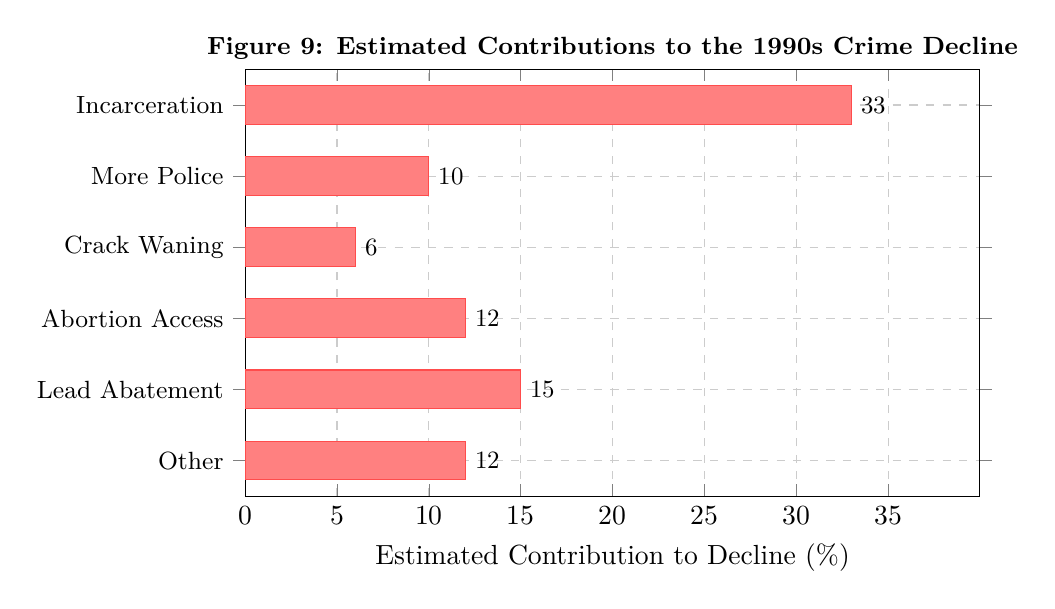
\begin{tikzpicture}
\begin{axis}[
    width=0.9\textwidth,
    height=7cm,
    title={\textbf{Figure 9: Estimated Contributions to the 1990s Crime Decline}},
    xbar,
    bar width=14pt,
    xlabel={Estimated Contribution to Decline (\%)},
    symbolic y coords={Other,Lead Abatement,Abortion Access,Crack Waning,More Police,Incarceration},
    ytick=data,
    yticklabel style={font=\small},
    xticklabel style={/pgf/number format/1000 sep={}},
    xmin=0, xmax=40,
    xtick={0,5,10,15,20,25,30,35},
    grid=major,
    grid style={dashed, gray!40},
    every axis title/.style={font=\bfseries\small, at={(0.5,1.05)}},
    nodes near coords,
    nodes near coords style={font=\small\bfseries, anchor=west},
]
\addplot[fill=red!50, draw=red!70] coordinates {
(12,Other)
(15,Lead Abatement)
(12,Abortion Access)
(6,Crack Waning)
(10,More Police)
(33,Incarceration)
};
\end{axis}
\end{tikzpicture}
\caption*{\emph{Sources: Steven D.\ Levitt, ``Understanding Why Crime Fell in the 1990s,'' Journal of Economic Perspectives 18, no.\ 1 (2004): 163--190; Brennan Center for Justice, ``What Caused the Crime Decline?'' (2015); Rick Nevin (2007) for lead abatement estimates. Note: While incarceration contributed through temporary incapacitation, subsequent research (National Research Council, 2014) found sharply diminishing returns after 1990. The decline was overwhelmingly driven by non-carceral factors.}}
\end{figure}

\begin{figure}[ht]
\centering
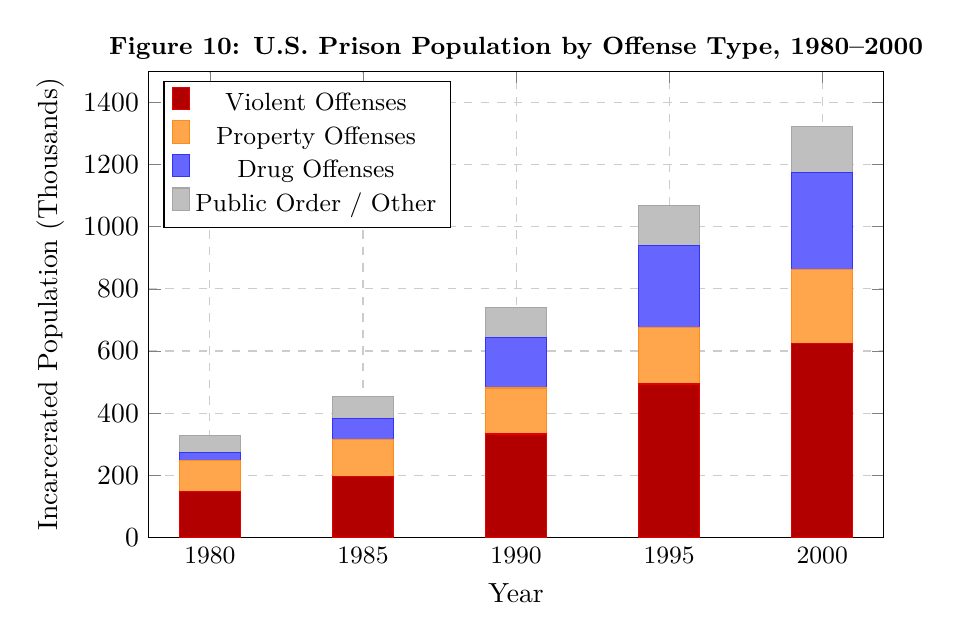
\begin{tikzpicture}
\begin{axis}[
    width=0.9\textwidth,
    height=7.5cm,
    title={\textbf{Figure 10: U.S.\ Prison Population by Offense Type, 1980--2000}},
    ybar stacked,
    bar width=22pt,
    xlabel={Year},
    ylabel={Incarcerated Population (Thousands)},
    symbolic x coords={1980,1985,1990,1995,2000},
    xtick=data,
    xticklabel style={font=\small, /pgf/number format/1000 sep={}},
    ymin=0, ymax=1500,
    ytick={0,200,400,600,800,1000,1200,1400},
    yticklabel style={/pgf/number format/1000 sep={}},
    grid=major,
    grid style={dashed, gray!40},
    every axis title/.style={font=\bfseries\small, at={(0.5,1.05)}},
    legend style={at={(0.02,0.98)}, anchor=north west, font=\small},
]
\addplot[fill=red!70!black, draw=red!90!black] coordinates {
    (1980, 148) (1985, 195) (1990, 333) (1995, 494) (2000, 624)
};
\addlegendentry{Violent Offenses}
\addplot[fill=orange!70, draw=orange!90] coordinates {
    (1980, 99) (1985, 120) (1990, 148) (1995, 182) (2000, 238)
};
\addlegendentry{Property Offenses}
\addplot[fill=blue!60, draw=blue!80] coordinates {
    (1980, 26) (1985, 68) (1990, 163) (1995, 265) (2000, 313)
};
\addlegendentry{Drug Offenses}
\addplot[fill=gray!50, draw=gray!70] coordinates {
    (1980, 56) (1985, 70) (1990, 96) (1995, 126) (2000, 147)
};
\addlegendentry{Public Order / Other}
\end{axis}
\end{tikzpicture}
\caption*{\emph{Sources: Bureau of Justice Statistics, ``Prisoners in [Year]'' series; Marc Mauer, ``Race to Incarcerate'' (rev.\ 2006); The Sentencing Project. Note: Drug offense incarceration grew by a factor of 12 between 1980 and 2000---from 26{,}000 to 313{,}000---the single fastest-growing category. This growth was driven by War on Drugs enforcement targeting low-level, nonviolent offenders in communities already devastated by deindustrialization.}}
\end{figure}

\subsection{\texorpdfstring{\textbf{Conclusion}}{Conclusion}}\label{conclusion}

The violent crime surge of the late twentieth century cannot be
understood through singular, monolithic narratives. It was a
multidimensional rupture caused by the volatile intersection of
macro-economic deindustrialization, the toxic environmental legacy of
lead exposure, the sudden influx of highly addictive narcotics, and the
lethal proliferation of concealable firearms.\\
Most critically, the surge was heavily concentrated in urban enclaves
that had been intentionally starved of capital and resources through
decades of systemic redlining and racial spatial engineering. When these
marginalized communities finally buckled under the weight of these
compounding crises, the American political establishment responded with
the only tool it had historically perfected: the carceral state.\\
By failing to address the systemic inequalities, economic voids, and
public health dimensions of the crisis, policies like the War on Drugs,
Broken Windows policing, and the 1994 Crime Bill leveraged the
desperation of terrorized communities to expand a prison-industrial
complex rooted in post-Civil War subjugation. While crime rates
eventually receded due to demographic shifts, the natural abatement of
the crack epidemic, and environmental detoxifications mandated by the
Clean Air Act, the legislative legacy of the era entrenched a system of
mass incarceration that continues to exact a devastating toll on
marginalized populations. Recognizing these interwoven frameworks
through rigorous, interdisciplinary analysis is essential to ensuring
that future public safety crises are met with holistic, systemic
investments rather than punitive extraction.

\nocite{*}
\printbibliography[title={Works cited},sorting=none]
\label{works-cited}

\end{document}
